\documentclass{article}
\usepackage{geometry}
\usepackage[utf8]{inputenc}
\usepackage{xcolor}
\usepackage{graphicx}
\usepackage{float,lscape}
\usepackage{listings}
\usepackage{color}
\usepackage{lipsum}% Used for dummy text.
\definecolor{titlepagecolor}{cmyk}{1,.60,0,.40}
\definecolor{namecolor}{cmyk}{1,.50,0,.10}
\definecolor{dkgreen}{rgb}{0,0.6,0}
\definecolor{gray}{rgb}{0.5,0.5,0.5}
\definecolor{mauve}{rgb}{0.58,0,0.82}
\lstset{frame=tb,
  language=Java,
  aboveskip=3mm,
  belowskip=3mm,
  showstringspaces=false,
  columns=flexible,
  basicstyle={\small\ttfamily},
  numbers=none,
  numberstyle=\tiny\color{gray},
  keywordstyle=\color{blue},
  commentstyle=\color{dkgreen},
  stringstyle=\color{mauve},
  breaklines=true,
  breakatwhitespace=true,
  tabsize=3
}
\title{Effective Field Method at Zero Temperature with Field Along Various Directions}
\author{Andrew Way}
\date{June 25th 2016}
%-----------------------------------------------------------------
\renewcommand{\topfraction}{.85}
\renewcommand{\bottomfraction}{.7}
\renewcommand{\textfraction}{.15}
\renewcommand{\floatpagefraction}{.66}
\renewcommand{\dbltopfraction}{.66}
\renewcommand{\dblfloatpagefraction}{.66}
\setcounter{topnumber}{9}
\setcounter{bottomnumber}{9}
\setcounter{totalnumber}{20}
\setcounter{dbltopnumber}{9}
\begin{document}

\maketitle

\tableofcontents

\clearpage
\section{Introduction}
    The effective field method was used to 3000 iterations (except where noted) to determine the 0 temperature states of 
    the 12x12x12 3D FCC kagome lattice while being subjected to a changing magnetic field along various field
    directions. 
    
    There are several types of runs which differ in either the starting state, the field direction, the maximum field
    to which the field was increased, and whether the field was then decreased after being saturated. When starting from a 
    ground state for any of the simulations included in this pdf, the ground state had characteristic angles theta = 0.206275 and phi = 3.11867.
    
    The purpose of these simulations was to observe the behaviour of the lattice's properties when subject to fields
    of various conditions.
    Analyses that was performed on the resulting data included the following:
    \begin{itemize}
     \item Plots of magnetization versus field
     \item Plots of energy versus field
     \item Composite plots of energy for both increasing and decreasing fields
     \item Composite plots of magnetization for both increasing and decreasing fields
     \item Snap shots of the characteristic 6 spins for each lattice at significant points of each simulation
     \item Determination of the number of ``unique'' spins that populate the lattice 
     \item Determination of the components of the unique spins
     \item Dot products of each of the 6 spins with their respective $``neighbors''$.  
    \end{itemize}
    
    Preliminary results providing insight on the causes of particular spin configurations due to application of field are also
    contained within the PDF. 
    
    \textbf{Note}: In all 6-spin snapshots, the spins are as such: A-Red, B-Green, C-Blue, D-Pink, E-Brown, F-Purple.
    Determining the number of unique spins that populate a particular lattice was not done for all simulations, but so
    far it seems that the lattice always maintains a 6 spin system, except during unstable periods in which the lattice
    undergoes a transition. It's likely that if the number of iterations used for EFM were increased and reran for
    transition phases the number of unique spins would probably reduce to 6. In other words, I think the system is changing too 
    quickly for EFM with 3000 iterations to properly find its ground state during transitions.
\clearpage
\section{(001) Increasing Field, Ground State}
\paragraph
\large
The 6 spins begin to transition to the planar state at H=0.0105 and achieves the planar state at H=0.0121.
The pink and brown spins swap positions, as do the blue and purple spins, as the field is increased beyond the planar state. 
The spins gradually align with the 001 field direction, until approximately at 0.14 the lattice becomes saturated and
the red and green and spins become parallel to the field direction. 
\begin{figure}[ht]
\centering
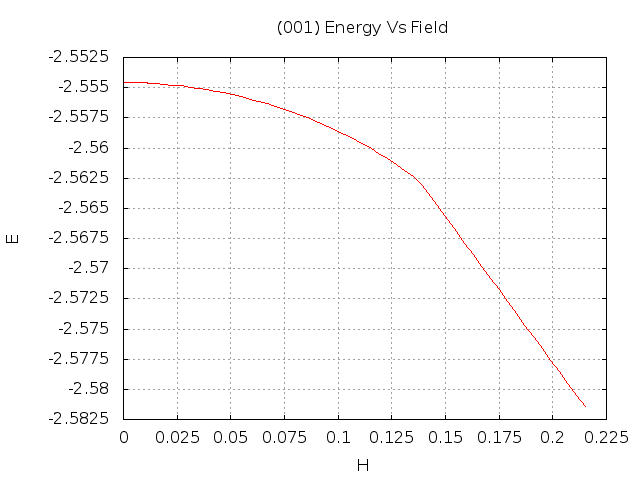
\includegraphics[scale=0.3]{HVariedData/Increasing/001Einc.png}
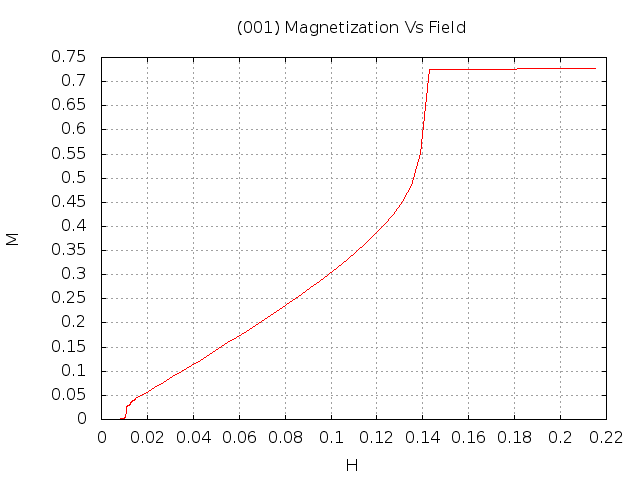
\includegraphics[scale=0.3]{HVariedData/Increasing/001Minc.png}
\end{figure}
\begin{figure}[ht]
\centering
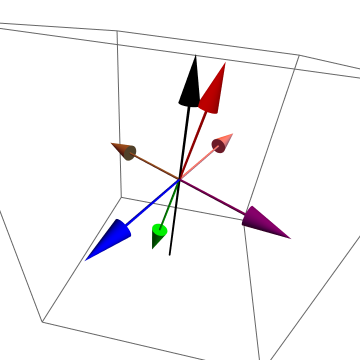
\includegraphics[scale=0.3]{HVariedData/Pictures/001Inc1.png}
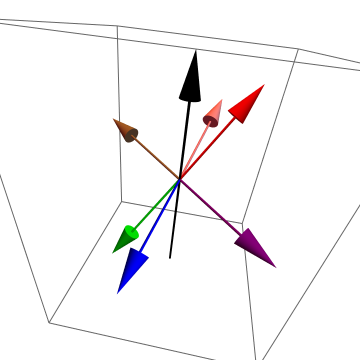
\includegraphics[scale=0.3]{HVariedData/Pictures/001Inc106.png}
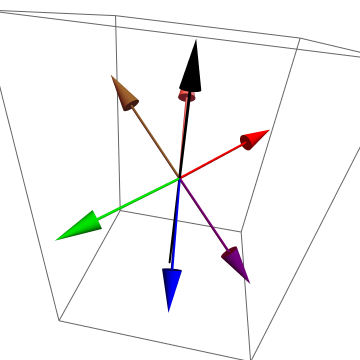
\includegraphics[scale=0.3]{HVariedData/Pictures/001Inc122.png}
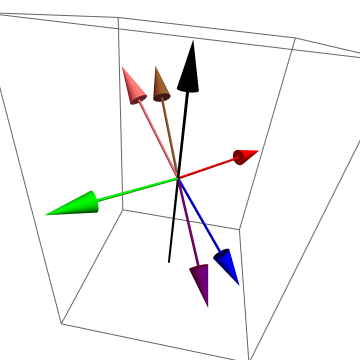
\includegraphics[scale=0.3]{HVariedData/Pictures/001Inc151.png}
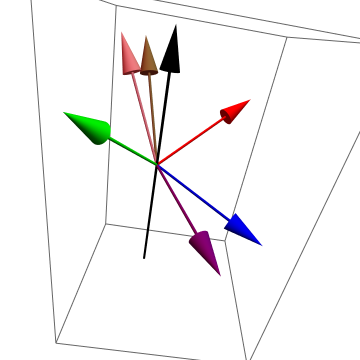
\includegraphics[scale=0.3]{HVariedData/Pictures/001Inc30S.png}
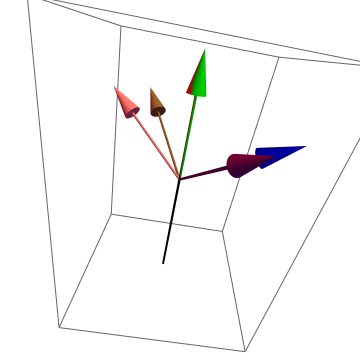
\includegraphics[scale=0.3]{HVariedData/Pictures/001Inc35S.png}
\caption{Snap shots of the 6 characteristic spins at H=0, 0.0105, 0.0121, 0.0150, 0.131, 0.151. The black arrow
indicates the direction of the field. In the dot product graph, AB dot product goes to zero once the lattice 
is saturated. This agrees with A and B (red and green) lining up in the above snapshots.}
\end{figure}
\clearpage

\section{(001) Decreasing Field, Ground State}
\paragraph
\large
The lattice leaves the saturated state at a field lower than what was required to induce it while increasing the field.
This transition from saturation occurs at approximately H=0.13, compared to the transition to saturation at H=0.14 when increasing the field. %Description here
The spins gradually unalign and rest in a planar state at zero field, and is characterized by the groundstate angles theta=89.9 degrees and phi=44.94 degrees.
\begin{figure}[ht]
\centering
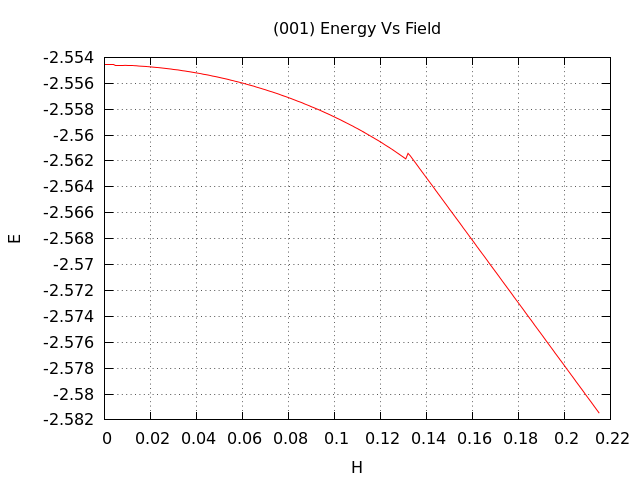
\includegraphics[scale=0.3]{HVariedData/Decreasing/001Edec.png}
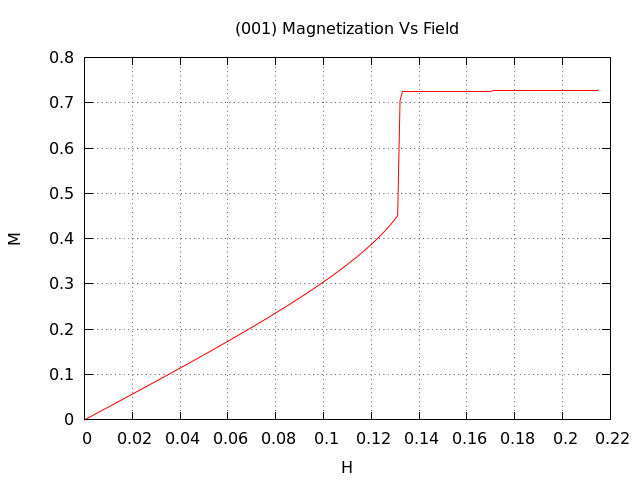
\includegraphics[scale=0.3]{HVariedData/Decreasing/001Mdec.png}
\end{figure}
\begin{figure}[ht]
\centering
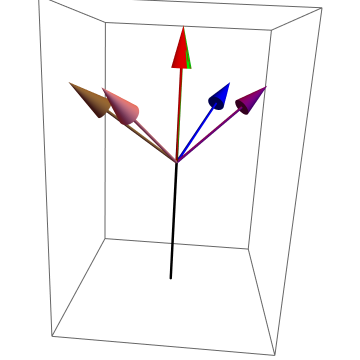
\includegraphics[scale=0.37]{HVariedData/Pictures/001Dec1.png}
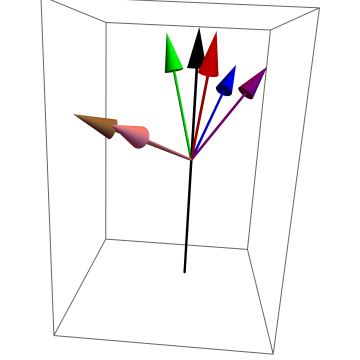
\includegraphics[scale=0.37]{HVariedData/Pictures/001Dec84.png}
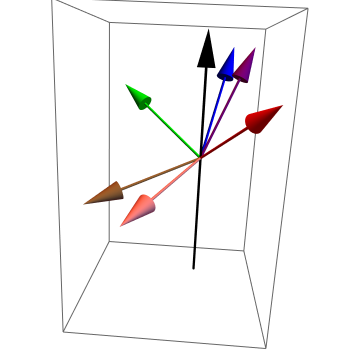
\includegraphics[scale=0.37]{HVariedData/Pictures/001Dec86.png}
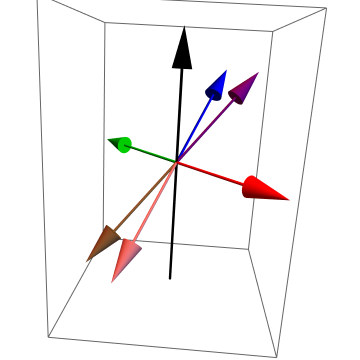
\includegraphics[scale=0.37]{HVariedData/Pictures/001Dec216.png}
\caption{Snapshots at H=0.215, 0.132, 0.130, 0}
\end{figure}

\begin{figure}[ht]
\centering
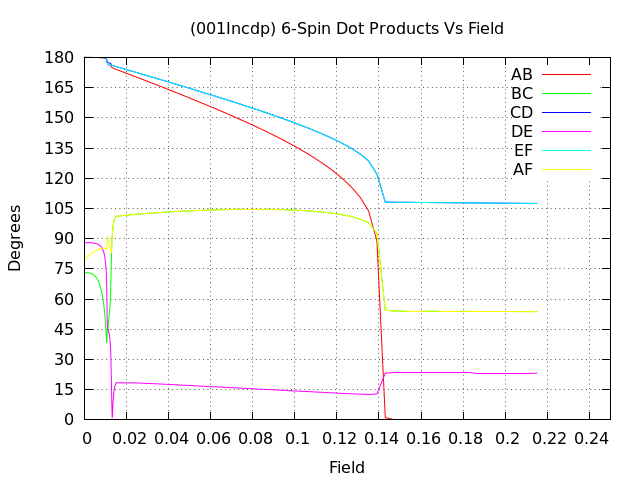
\includegraphics[scale=0.55]{HVariedData/Pictures/001Incdp.png}
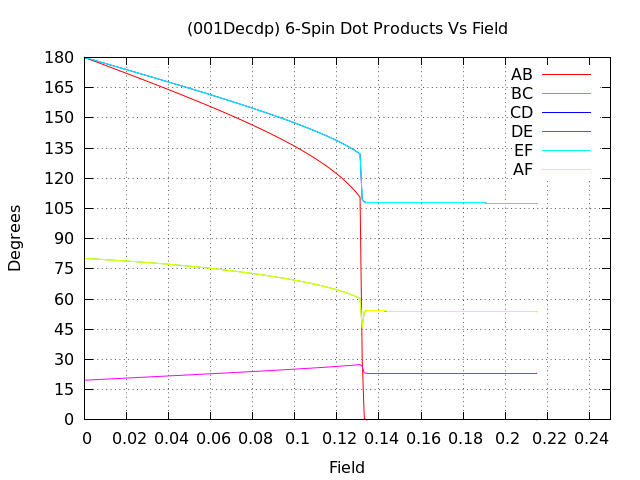
\includegraphics[scale=0.55]{HVariedData/Pictures/001Decdp.png}
\caption{Dot products between the characteristic spins for both increasing and decreasing field.}
\end{figure}

\begin{figure}[ht]
\centering
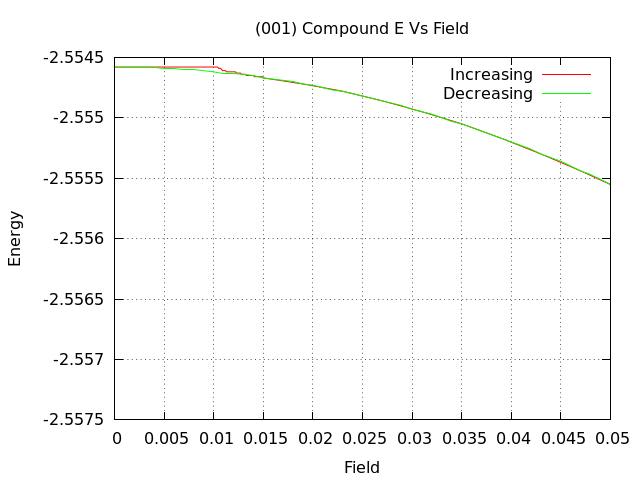
\includegraphics[scale=0.5]{HVariedData/compoundEM/001Ecompound.png}
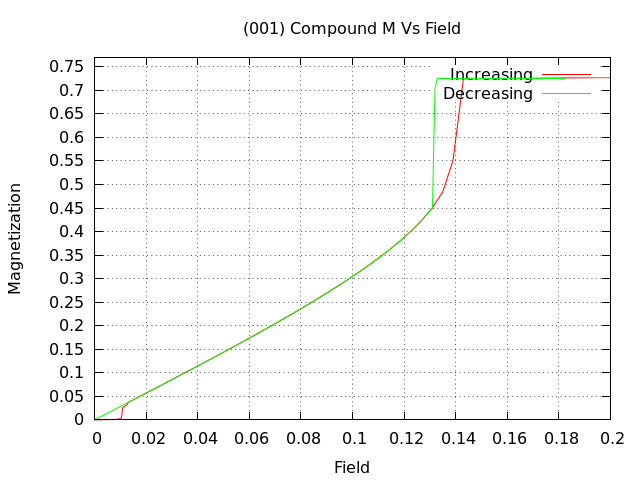
\includegraphics[scale=0.5]{HVariedData/compoundEM/001Mcompound.png}
\caption{Composite graphs of energy and magnetization for both decreasing and increasing field magnitude. Note the
different scales for the energy and magnetization graph. This is because plotting energy vs field on a graph
which has an xrange of 0.2 reduces the ability to see any difference in the energy curves. This was done for all 
composite graphs.}
\end{figure}
\clearpage


\section{(010) Increasing Field, Ground State}
\paragraph
\large
The lattice begins to undergo a transition at 0.0110. At 0.0114 the planar state is achieved. Similar to 001,
two pairs of spins begin to swap positions at around 0.015, though the pairs consist of spins different from 001.
The blue and green spins and red and pink spins appear to be swapping positions, but never do. The spins gradually
align with the 010 direction until at approximately H=0.14 the lattice becomes saturated and the purple and brown spins
become parallel to the field direction.%Description here

\begin{figure}[ht]
\centering
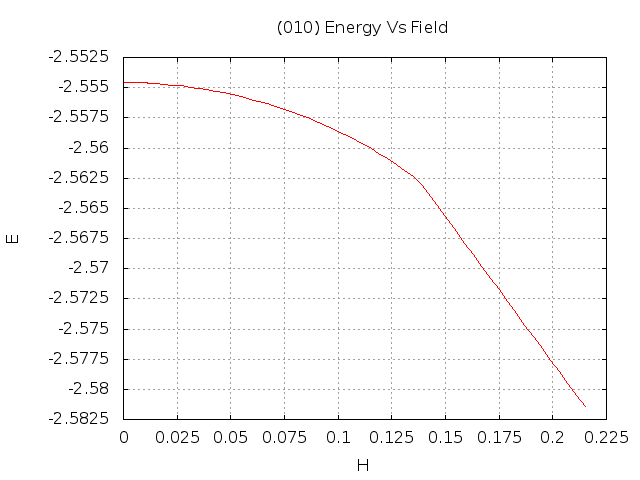
\includegraphics[scale=0.3]{HVariedData/Increasing/010Einc.png}
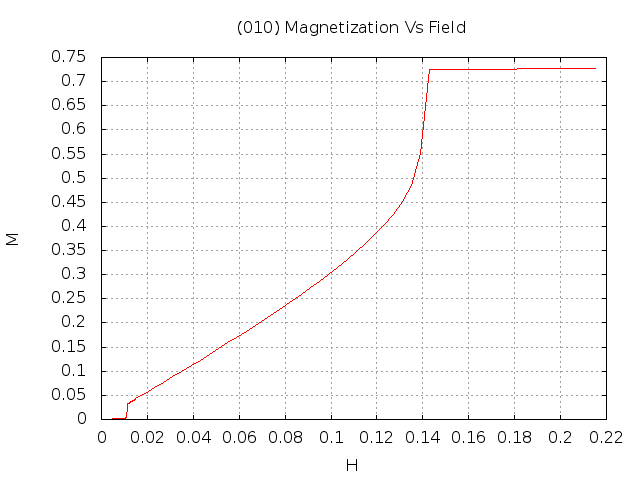
\includegraphics[scale=0.3]{HVariedData/Increasing/010Minc.png}
\end{figure}
\begin{figure}[ht]
\centering
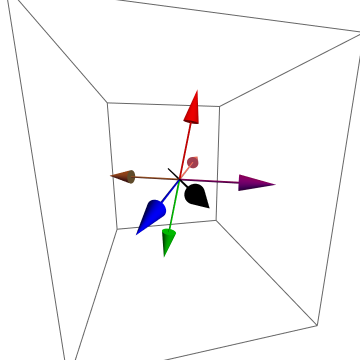
\includegraphics[scale=0.3]{HVariedData/Pictures/010Inc1.png}
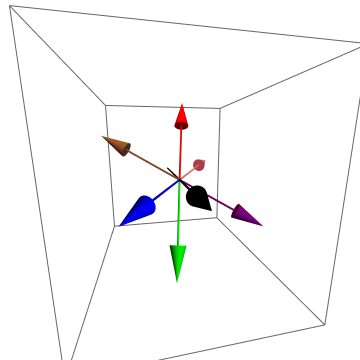
\includegraphics[scale=0.3]{HVariedData/Pictures/010Inc111.png}
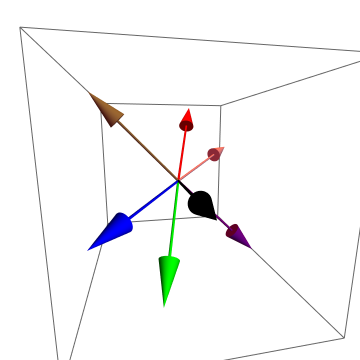
\includegraphics[scale=0.3]{HVariedData/Pictures/010Inc118.png}
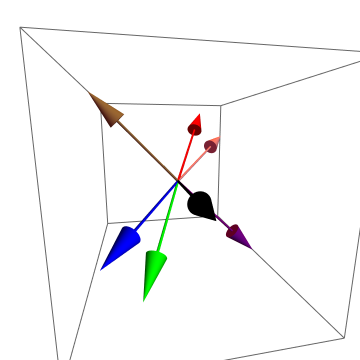
\includegraphics[scale=0.3]{HVariedData/Pictures/010Inc151.png}
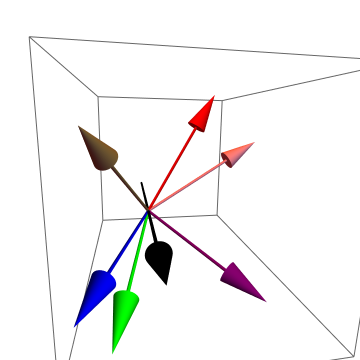
\includegraphics[scale=0.3]{HVariedData/Pictures/010Inc32S.png}
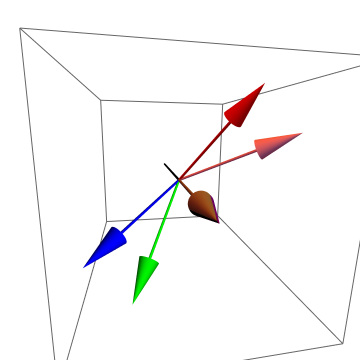
\includegraphics[scale=0.3]{HVariedData/Pictures/010Inc33S.png}
\caption{Snapshots at H=0, 0.0110, 0.0117, 0.0150, 0.139, 0.179 }
\end{figure}

\clearpage

\section{(010) Decreasing Field, Ground State}
\paragraph
\large
The lattice is released from saturation at approximately field=0.13, a field magnitude lower than the increasing field required
to induce saturation. The spins gradually unalign with the decreasing field, and rest at a zero field planar state
characterized by angles theta=52.7 degrees and phi=-117.275 degrees.%Description here

\begin{figure}[ht]
\centering
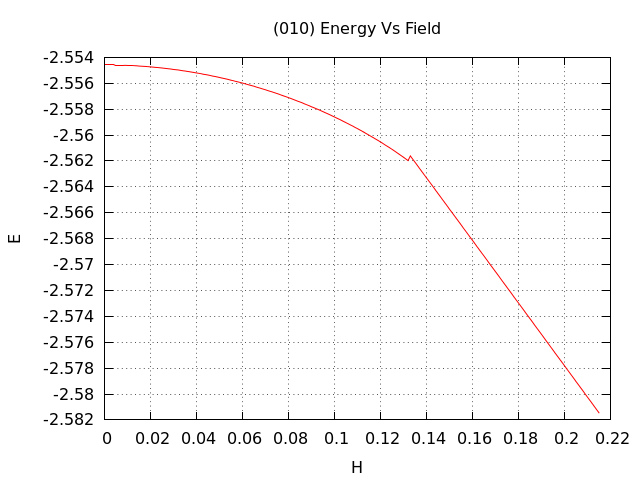
\includegraphics[scale=0.3]{HVariedData/Decreasing/010Edec.png}
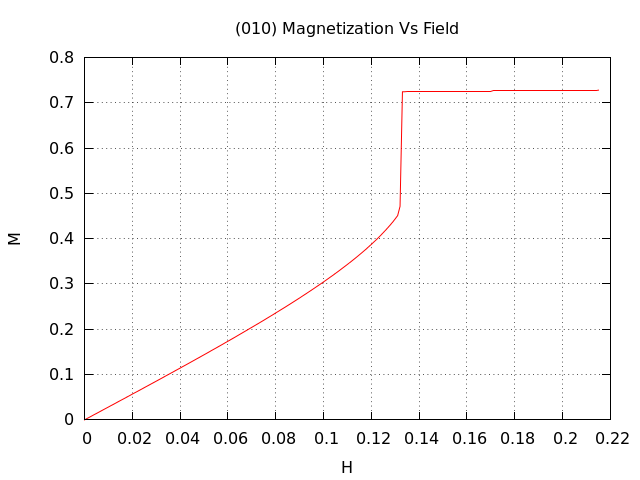
\includegraphics[scale=0.3]{HVariedData/Decreasing/010Mdec.png}
\end{figure}
\begin{figure}[ht]
\centering
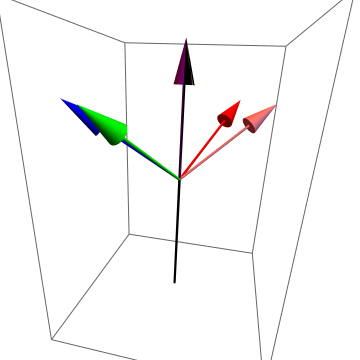
\includegraphics[scale=0.35]{HVariedData/Pictures/010Dec1.png}
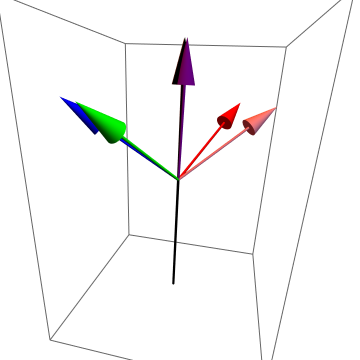
\includegraphics[scale=0.35]{HVariedData/Pictures/010Dec83.png}
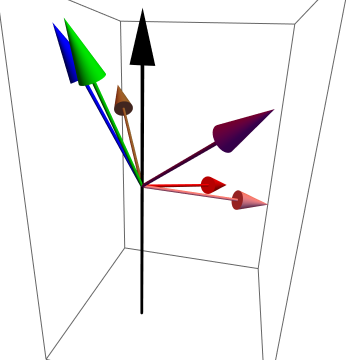
\includegraphics[scale=0.35]{HVariedData/Pictures/010Dec84.png}
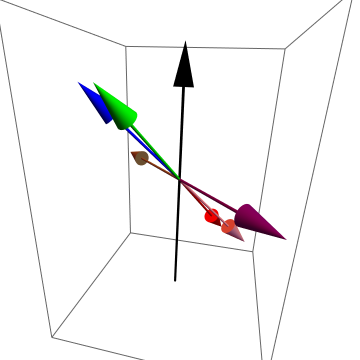
\includegraphics[scale=0.35]{HVariedData/Pictures/010Dec216.png}
\caption{Snapshots of the 6 characteristic spins at H=0.215, 0.132, 0.131, 0. While the field arrow is pointing up,
it is still pointing in the 010 direction.}
\end{figure}
\clearpage

\begin{figure}[ht]
\centering
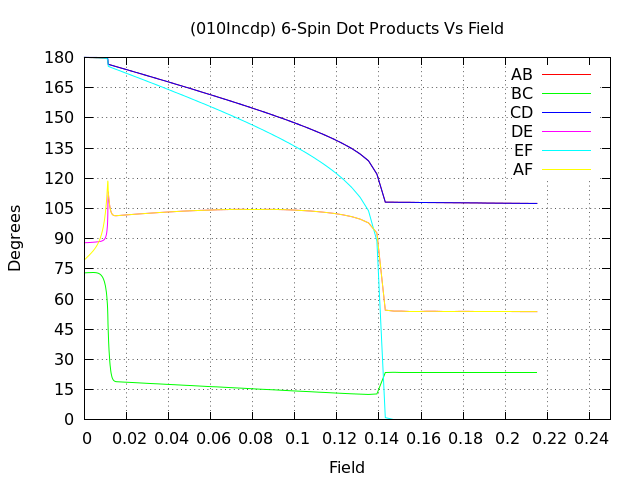
\includegraphics[scale=0.5]{HVariedData/Pictures/010Incdp.png}
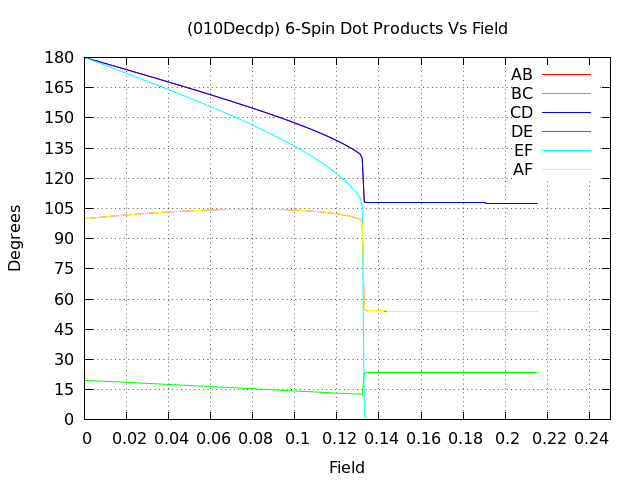
\includegraphics[scale=0.5]{HVariedData/Pictures/010Decdp.png}
\caption{Dot products between the characteristic spins for both increasing and decreasing field.}
\end{figure}
\clearpage

\begin{figure}[ht]
\centering
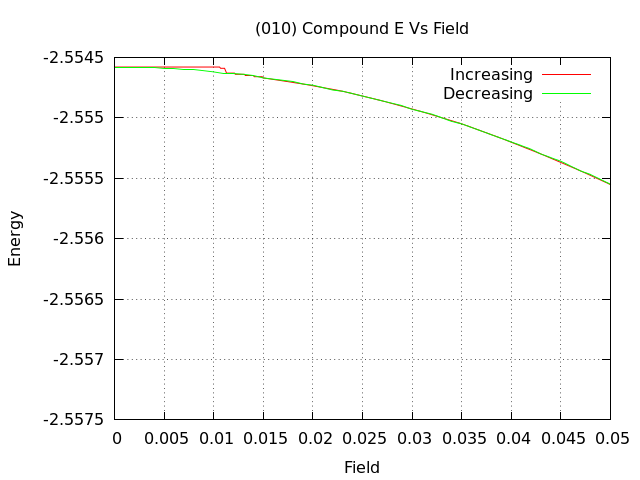
\includegraphics[scale=0.6]{HVariedData/compoundEM/010Ecompound.png}
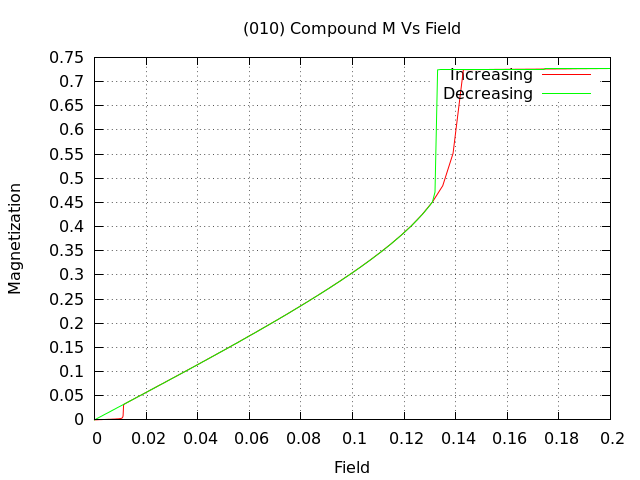
\includegraphics[scale=0.6]{HVariedData/compoundEM/010Mcompound.png}
\caption{Composite graphs of energy and magnetization for both decreasing and increasing field magnitude.}
\end{figure}
\clearpage
\section{(011) Increasing Field, Ground State}
\paragraph
\large
The lattice begins to transition at approximately 0.007. At 0.0074 the planar state is achieved. At 0.0093, the 
pink and red spins swap position, and the blue and green spins swap position. As the field is increased further to 0.0115,
the green and brown spins begin to swap positions. At 0.143, this is achieved. Once saturated, no spins are parallel
with the field direction.%Description here

\begin{figure}[ht]
\centering
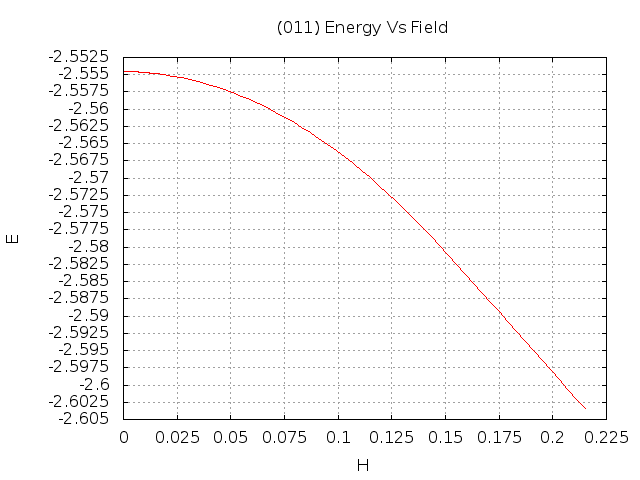
\includegraphics[scale=0.3]{HVariedData/Increasing/011Einc.png}
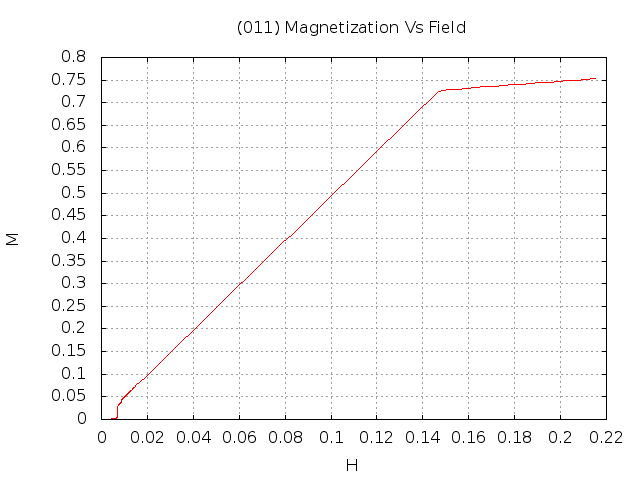
\includegraphics[scale=0.3]{HVariedData/Increasing/011Minc.png}
\end{figure}
\begin{figure}[ht]
\centering
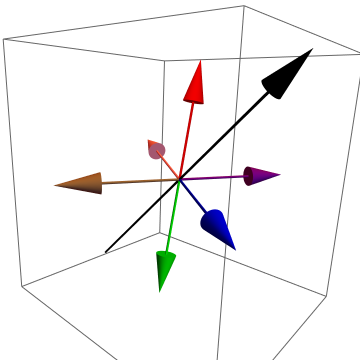
\includegraphics[scale=0.3]{HVariedData/Pictures/011Inc1.png}
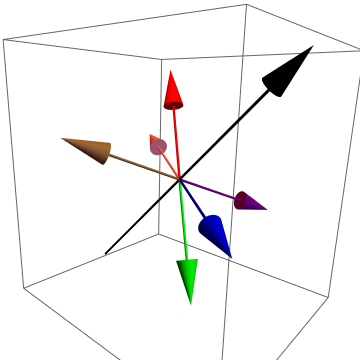
\includegraphics[scale=0.3]{HVariedData/Pictures/011Inc67.png}
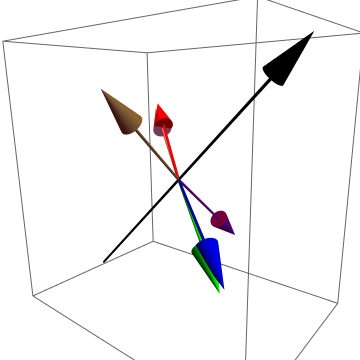
\includegraphics[scale=0.3]{HVariedData/Pictures/011Inc82.png}
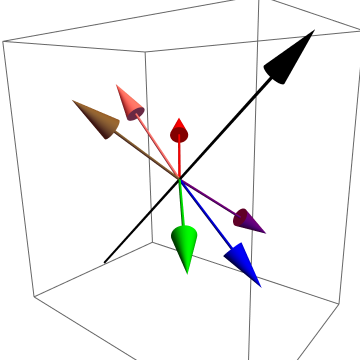
\includegraphics[scale=0.3]{HVariedData/Pictures/011Inc94.png}
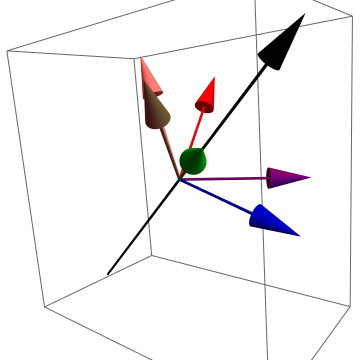
\includegraphics[scale=0.3]{HVariedData/Pictures/011Inc26S.png}
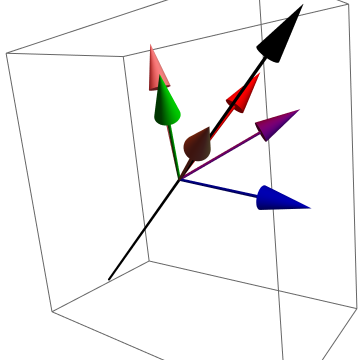
\includegraphics[scale=0.3]{HVariedData/Pictures/011Inc39S.png}
\caption{Snapshots at H=0, 0.0066, 0.0082, 0.0094, 0.115, 0.167}
\end{figure}

\clearpage

\section{(011) Decreasing Field, Ground State}
\paragraph
\large
As the field is decreased to 0.134, the brown and green spins swap positions again. All 6 spins gradually unalign
with the field until they reach a zero field planar state characterized by angles theta=69.33 degrees and phi=-139.133 degrees.%Description here

\begin{figure}[ht]
\centering
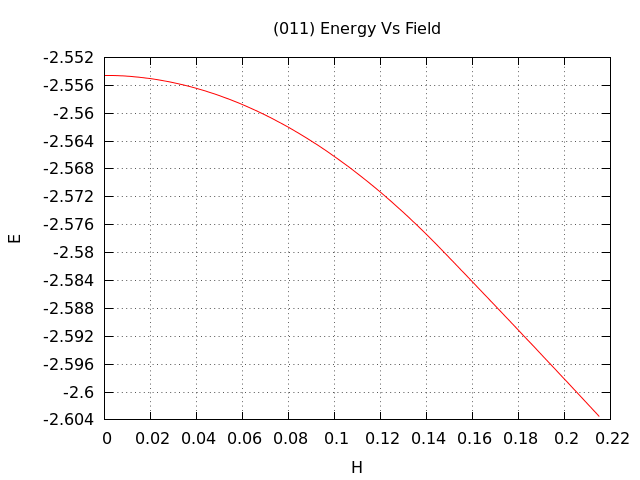
\includegraphics[scale=0.3]{HVariedData/Decreasing/011Edec.png}
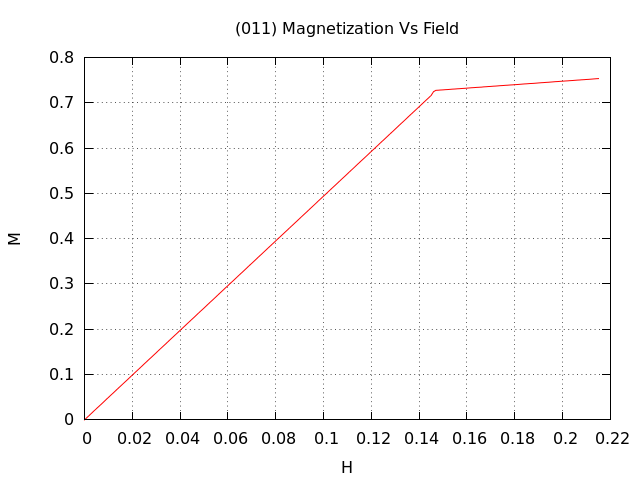
\includegraphics[scale=0.3]{HVariedData/Decreasing/011Mdec.png}
\end{figure}
\begin{figure}[ht]
\centering
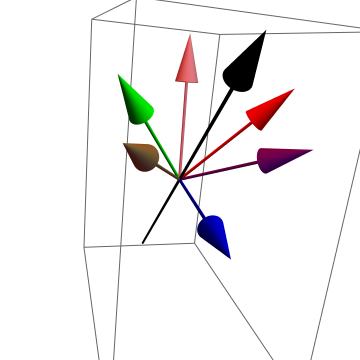
\includegraphics[scale=0.37]{HVariedData/Pictures/011Dec1.png}
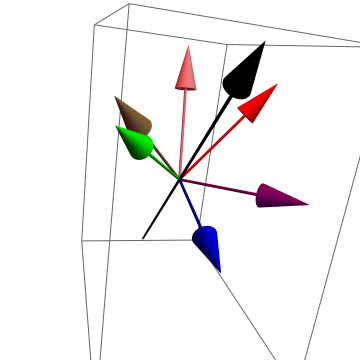
\includegraphics[scale=0.37]{HVariedData/Pictures/011Dec82.png}
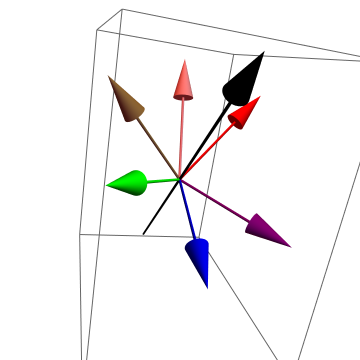
\includegraphics[scale=0.37]{HVariedData/Pictures/011Dec122.png}
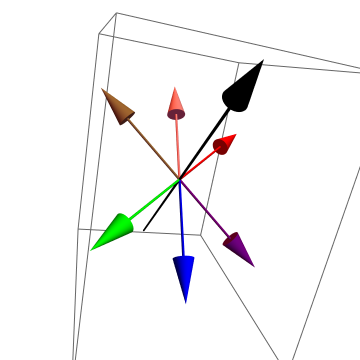
\includegraphics[scale=0.37]{HVariedData/Pictures/011Dec216.png}
\caption{Snapshots at H=0.215, 0.134, 0.094, 0}
\end{figure}

\begin{center}
\begin{figure}
\centering
\includegraphics[scale=0.5]{HVariedData/Pictures/011Incdp.png}
\includegraphics[scale=0.5]{HVariedData/Pictures/011Decdp.png}
\caption{Dot products between the characteristic spins for both increasing and decreasing field.}
\end{figure}
\end{center}
\clearpage

\begin{figure}[ht]
\centering
\includegraphics[scale=0.6]{HVariedData/compoundEM/011Ecompound.png}
\includegraphics[scale=0.6]{HVariedData/compoundEM/011Mcompound.png}
\caption{Composite graphs of energy and magnetization for both decreasing and increasing field magnitude.}
\end{figure}
\clearpage
\section{(100) Increasing Field, Ground State}
\paragraph
\large
%\addcontentsline{toc}{section}{Unnumbered Section}
Two inflection points are observed in the magnetization graph. There are two inflection points in the
energy graph as well, however they are not as obvious. A planar state is achieved at 0.0041. Between 0.0041 and
0.0064, the brown and green spins become closer to one another, as do the red and purple spins. The pink and blue
spins remain fixed. The spins gradually align with the field, until it suddenly snaps into its final position where
the blue and pink spins point in the same direction, in addition to lying within the xy plane. The lattice is
saturated beyond this point. 
\begin{figure}[h]
 \centering 
\includegraphics[scale=0.3]{100/E000to005G.png}
\includegraphics[scale=0.3]{100/M000to005G.png}
\caption{Energy vs increasing field and Magnetization versus increasing field}
\end{figure}
\begin{figure}[ht]
\centering
\includegraphics[scale=0.28]{100/1S000to005G.png}
\includegraphics[scale=0.28]{100/39S000to005G.png}
\includegraphics[scale=0.28]{100/42S000to005G.png}
\includegraphics[scale=0.28]{100/55S000to005G.png}
\includegraphics[scale=0.28]{100/419S000to005G.png}
\includegraphics[scale=0.28]{100/466S000to005G.png}
\includegraphics[scale=0.28]{100/467S000to005G.png}
\includegraphics[scale=0.28]{100/501S000to005G.png}
\caption{H=0, 0.0038, 0.0041, 0.0054, 0.0418, 0.0465, 0.0466 and 0.05}
\end{figure}

\clearpage
\section{(100) Decreasing Field, Ground State}
\paragraph
\large
As the field is decreased, the spins are released from the saturated state, and return to the typically observed
planar state, that gradually unaligns with the field direction as the field is decreased. Finally, the spins return
to a full planar state, and not the original zero field ground state. The starting configuration of this run
was not the final configuration of the (100) Increasing Field, Ground State run, but the same zero field ground state
that the (100) Increasing Field, Ground state started from. The final configuration is characterized by angles theta=51.63 degrees 
and phi=154.414 degrees.
\begin{figure}[ht]
 \centering 
\includegraphics[scale=0.3]{100/E005to000G.png}
\includegraphics[scale=0.3]{100/M005to000G.png}
\caption{Energy vs decreasing field and Magnetization versus decreasing field}
\end{figure}
\begin{figure}[ht]
\centering
\includegraphics[scale=0.24]{100/1S005to000G.png}
\includegraphics[scale=0.24]{100/3S005to000G.png}
\includegraphics[scale=0.24]{100/55S005to000G.png}
\includegraphics[scale=0.24]{100/56S005to000G.png}
\includegraphics[scale=0.24]{100/129S005to000G.png}
\includegraphics[scale=0.24]{100/501S005to000G.png}
\caption{H=0.05, 0.0498, 0.0446, 0.0445, 0.0372, and 0. It can be seen that the pink and blue spins have not yet
entirely lined up with the field vector in the first picture, but they have in the second picture. This indicates that
simply using a zero field groundstate and subjecting it to a high field immediately with only 3000 steps does not yield
the true state for that field.}
\end{figure}
\clearpage

\begin{figure}[ht]
\centering
\includegraphics[scale=0.5]{HVariedData/Pictures/100Decdp.png}
\includegraphics[scale=0.5]{HVariedData/Pictures/100Incdp.png}
\caption{Dot products between the characteristic spins for both increasing and decreasing field. The data only continues
to a low field relative to other simulations due to the saturation field occuring so early. A simulation continuing
this run is currently being worked on.}
\end{figure}
\clearpage

\begin{figure}[ht]
\centering
\includegraphics[scale=0.6]{HVariedData/compoundEM/100Ecompound.png}
\includegraphics[scale=0.6]{HVariedData/compoundEM/100Mcompound.png}
\caption{Composite graphs of energy and magnetization for both decreasing and increasing field magnitude.}
\end{figure}
\clearpage

\begin{figure}[ht]
\centering
\includegraphics[scale=0.5]{100/000to005Freq.png}
\includegraphics[scale=0.5]{100/005to000Freq.png}
\caption{The number of unique spins within the lattice. The labelling is
not clear, and not consistent throughout this pdf since these graphs were not completely finished at the time of making the pdf. The first
graph's x axis begins at H=0, and ends at H=0.05, and depicts the number of spins within the system during an increasing field. The second
is for decreasing field.}
\end{figure}
\clearpage

\section{(100) Increasing Field, Random State}
The energy drops very quickly at near zero field, which is likely because of insufficient number of iterations. Two
points of inflection are observed. The transition of the spins is very similar to starting from a ground state.
\begin{figure}[h]
 \centering 
\includegraphics[scale=0.3]{100/E000to005R.png}
\includegraphics[scale=0.3]{100/M000to005R.png}
\caption{Energy vs increasing field and Magnetization versus increasing field}
\end{figure}
\begin{figure}[ht]
\centering
\includegraphics[scale=0.27]{100/1S000to005R.png}
\includegraphics[scale=0.27]{100/2S000to005R.png}
\includegraphics[scale=0.27]{100/48S000to005R.png}
\includegraphics[scale=0.27]{100/54S000to005R.png}
\includegraphics[scale=0.27]{100/55S000to005R.png}
\includegraphics[scale=0.27]{100/411S000to005R.png}
\includegraphics[scale=0.27]{100/467S000to005R.png}
\includegraphics[scale=0.27]{100/501S000to005R.png}
\caption{H = 0.00, 0.0001, 0.0047, 0.0053, 0.0054, 0.0410, 0.0466, 0.05}
\end{figure}
\clearpage

\section{(100) Decreasing Field, Random State}
The lattice starts off in a planar state. As the field is decreased, spins gradually unalign with the field. 
Suddenly, at 0.0455, the spins snap back into a slight realigned planar state. Another sudden readjustment
is observed at 0.025. Finally, the spins return a full planar state at 0 field. The red and brown spins
swap positions as the field lowers, as do the green and purple spins. This is likely a result of insufficient EFM iterations.
\begin{figure}[h]
 \centering 
\includegraphics[scale=0.3]{100/E005to000R.png}
\includegraphics[scale=0.3]{100/M005to000R.png}
\caption{Energy vs decreasing field and Magnetization versus decreasing field}
\end{figure}
\begin{figure}[ht]
\centering
\includegraphics[scale=0.3]{100/1S005to000R.png}
\includegraphics[scale=0.3]{100/41S005to000R.png}
\includegraphics[scale=0.3]{100/46S005to000R.png}
\includegraphics[scale=0.3]{100/244S005to000R.png}
\includegraphics[scale=0.3]{100/245S005to000R.png}
\includegraphics[scale=0.3]{100/501S005to000R.png}
\caption{H = 0.05, 0.0460, 0.0455, 0.0257, 0.0256, 0.00.}
\end{figure}
\clearpage

\begin{figure}[ht]
\centering
\includegraphics[scale=0.5]{HVariedData/Pictures/100DecdpR.png}
\includegraphics[scale=0.5]{HVariedData/Pictures/100IncdpR.png}
\caption{Dot products between the characteristic spins for both increasing and decreasing field. The data only continues
to a low field relative to other simulations due to the saturation field occuring so early. A simulation continuing
this run is currently being worked on.}
\end{figure}
\clearpage


\begin{figure}[ht]
\centering
\includegraphics[scale=0.5]{100/000to005RFreq.png}
\includegraphics[scale=0.5]{100/005to000RFreq.png}
\caption{At high field, while decreasing it, a huge number of $``unique''$ spins was observed. When looking through one of the configuration
files, most spins only agreed with some other spins to at most 1 decimal place. The program that determines whether
a spin is unique considers a spin to be unique when it doesn't agree with any previously found spin up to at least two decimal 
places. Hence, the large number of unique spins present.The plateau in the middle is actually just false data I put
into the text file, since I cancelled the program since it was taking a very long time. I reran the program from around
H = 0.0250 to 0, and found that the lattice in this field range always had 6 unique spins.}
\end{figure}
\clearpage
\section{(101) Increasing Field, Ground State}
\paragraph
\large
The lattice begins to undergo a transition to a planar state at 0.0055, where it is achieved at 0.0060. At 0.0115 
the purple and red spins and green and brown spins begin to swap positions, which is complete at 0.0128. At approximately
0.14, the green and pink spins swap position. Upon swapping, the lattice becomes saturated.%Description here

\begin{figure}[ht]
\centering
\includegraphics[scale=0.3]{HVariedData/Increasing/101Einc.png}
\includegraphics[scale=0.3]{HVariedData/Increasing/101Minc.png}
\end{figure}
\begin{figure}[ht]
\centering
\includegraphics[scale=0.29]{HVariedData/Pictures/101Inc1.png}
\includegraphics[scale=0.29]{HVariedData/Pictures/101Inc56.png}
\includegraphics[scale=0.29]{HVariedData/Pictures/101Inc61.png}
\includegraphics[scale=0.29]{HVariedData/Pictures/101Inc116.png}
\includegraphics[scale=0.29]{HVariedData/Pictures/101Inc128.png}
\includegraphics[scale=0.29]{HVariedData/Pictures/101Inc32S.png}
\includegraphics[scale=0.29]{HVariedData/Pictures/101Inc38S.png}
\caption{H=0, 0.0055, 0.0060, 0.0115, 0.0128, 0.0.139, 0.163}
\end{figure}
\clearpage

\section{(101) Decreasing Field, Ground State}
\paragraph
\large
When decreasing the field, instead of the pink and green re-swapping positions the
blue and red spins, the spins that mirror them, swap positions at approximately 0.137. The final configuration
is characterized by angles theta=110.826 degrees and phi=49.1513 degrees.%Description here
\begin{figure}[ht]
\centering
\includegraphics[scale=0.3]{HVariedData/Decreasing/101Edec.png}
\includegraphics[scale=0.3]{HVariedData/Decreasing/101Mdec.png}
\end{figure}
\begin{figure}[ht]
\centering
\includegraphics[scale=0.37]{HVariedData/Pictures/101Dec1.png}
\includegraphics[scale=0.37]{HVariedData/Pictures/101Dec79.png}
\includegraphics[scale=0.37]{HVariedData/Pictures/101Dec125.png}
\includegraphics[scale=0.37]{HVariedData/Pictures/101Dec216.png}
\caption{Snapshots at H=0.2150, 0.137, 0.09, 0}
\end{figure}

\begin{center}
\begin{figure}
\centering
\includegraphics[scale=0.5]{HVariedData/Pictures/101Incdp.png}
\includegraphics[scale=0.5]{HVariedData/Pictures/101Decdp.png}
\caption{Dot products between the characteristic spins for both increasing and decreasing field.}
\end{figure}
\end{center}
\clearpage

\begin{figure}[ht]
\centering
\includegraphics[scale=0.6]{HVariedData/compoundEM/101Ecompound.png}
\includegraphics[scale=0.6]{HVariedData/compoundEM/101Mcompound.png}
\caption{Composite graphs of energy and magnetization for both decreasing and increasing field magnitude.}
\end{figure}
\clearpage

%110 ----------------------------------------------------------------------------------------------
\pagebreak
\section{(110) Increasing Field, Ground State}
Two inflection points are evident in the graphs of energy and magnetization, indicating the occurence of a sudden
change in orientation of the spins. The first inflection point occurs at H~0.005, at which the spins snap into a 
planar state. The second occurs at H~0.009, where another planar state forms but oriented in a different direction. This 
is the result of the red and purple spins swapping positions, and the brown and green spins swapping positions. 
\begin{figure}[ht]
 \centering 
\includegraphics[scale=0.3]{HVariedData/Increasing/110EInc.png}
\includegraphics[scale=0.3]{HVariedData/Increasing/110Minc.png}
\caption{Energy vs increasing field and Magnetization versus increasing field}
\end{figure}
\begin{figure}[ht]
\centering
\includegraphics[scale=0.28]{110/1S000to005G.png}
\includegraphics[scale=0.28]{110/47S000to005G.png}
\includegraphics[scale=0.28]{110/50S000to005G.png}
\includegraphics[scale=0.28]{110/96S000to005G.png}
\includegraphics[scale=0.28]{110/501S000to005G.png}
\includegraphics[scale=0.28]{HVariedData/Pictures/110Inc40S.png}
\includegraphics[scale=0.28]{HVariedData/Pictures/110Inc51S.png}
\caption{Snapshots of the 6 characteristic spins of the lattice at H=0, 0.0046, 0.0049, 0.0095, 0.05, 0.089, and 0.1}
\end{figure}
\clearpage

\section{(110) Decreasing Field, Ground State}
Similar to starting with a high field in the 111 direction, the spins are in a planar state that is
aligned with the field. When the field is lowered, the spins are stuck in a planar state. In the first
snapshot of the spins, the brown and green spins are partially aligned. This is likely due to insufficient
number of iterations for EFM. The final configuration has characteristic angles theta=90.096 degrees and phi=135.034 degrees.
The starting configuration of this run
was not the final configuration of the (110) Increasing Field, Ground State run, but the same zero field ground state
that the (110) Increasing Field, Ground state started from.
\begin{figure}[h]
 \centering 
\includegraphics[scale=0.3]{HVariedData/Decreasing/110Edec.png}
\includegraphics[scale=0.3]{HVariedData/Decreasing/110Mdec.png}
\caption{Energy vs decreasing field and Magnetization versus decreasing field}
\end{figure}
\begin{figure}[ht]
\centering
\includegraphics[scale=0.3]{HVariedData/Pictures/110Dec1.png}
\includegraphics[scale=0.3]{HVariedData/Pictures/110Dec102.png}
\includegraphics[scale=0.3]{HVariedData/Pictures/110Dec122.png}
\includegraphics[scale=0.3]{HVariedData/Pictures/110Dec201.png}
\caption{Snapshots of the 6 characteristic spins of the lattice at H=0.2, 0.121, 0.101, and 0 }
\end{figure}
\clearpage

\begin{figure}[ht]
\centering
\includegraphics[scale=0.5]{HVariedData/Pictures/110Incdp.png}
\includegraphics[scale=0.5]{HVariedData/Pictures/110Decdp.png}
\caption{Dot products between the 6 characteristic spins of the lattice.}
\end{figure}
\clearpage

\begin{figure}[ht]
\centering
\includegraphics[scale=0.6]{HVariedData/compoundEM/110Ecompound.png}
\includegraphics[scale=0.6]{HVariedData/compoundEM/110Mcompound.png}
\caption{Composite graphs of energy and magnetization for both decreasing and increasing field magnitude.}
\end{figure}
\clearpage

\begin{figure}[ht]
\centering
\includegraphics[scale=0.5]{110/000to005Freq.png}
\includegraphics[scale=0.5]{110/005to000Freq.png}
\caption{As mentioned before, these graphs aren't finished. The top graph's x-axis begins at H=0, and ends at H=0.05.
The bottom graph's x-axis begins at H=0.05 and ends at H=0. }
\end{figure}
\clearpage

\section{(110) Increasing Field, Random State}
Very similar to beginning with the ground state, in that there are 2 transitions at approximately 0.0038 and 0.0075. The transformation of the 
6 spins is similar as well,
with the spins beginning in the groundstate, transition to a planar state, 2 pairs of spins rotate and switch places,
and the plane the spins lie in reorients itself. The spins then gradually align with the field.
\begin{figure}[ht]
 \centering 
\includegraphics[scale=0.3]{HVariedData/Increasing/110EIncR.png}
\includegraphics[scale=0.3]{HVariedData/Increasing/110MincR.png}
\caption{Energy vs increasing field and Magnetization versus increasing field}
\end{figure}
\begin{figure}[ht]
\centering
\includegraphics[scale=0.33]{110/1S000to005R.png}
\includegraphics[scale=0.33]{110/69S000to005R.png}
\includegraphics[scale=0.33]{110/82S000to005R.png}
\includegraphics[scale=0.33]{110/501S000to005R.png}
\caption{Snapshots of the 6 spins at H = 0.00, 0.0068, 0.0081, and 0.05}
\end{figure}
\clearpage

\section{(110) Decreasing Field, Random State}
A sudden transition occurs at approximately 0.022. The green and pink spins swap places with another, and the blue
and red spins also follow this swap. It's possible this transition only occurs because there is insufficient
steps being used for EFM, as was the case with applying the field in the 111 direction. Any transitions disappeared
when increasing the number of steps from 2000 to 3000 steps when decreasing the field with a random initial 
configuration. 
\begin{figure}[ht]
 \centering 
\includegraphics[scale=0.3]{110/E005to000R.png}
\includegraphics[scale=0.3]{110/M005to000R.png}
\caption{Energy vs decreasing field and Magnetization versus decreasing field}
\end{figure}
\begin{figure}[ht]
\centering
\includegraphics[scale=0.33]{110/1S005to000R.png}
\includegraphics[scale=0.33]{110/241S005to000R.png}
\includegraphics[scale=0.33]{110/300S005to000R.png}
\includegraphics[scale=0.33]{110/501S005to000R.png}
\caption{Snapshots at H=0.05, H=0.0260, 0.0201, and 0.}
\end{figure}
\clearpage

\begin{figure}[ht]
\centering
\includegraphics[scale=0.5]{HVariedData/Pictures/110IncdpR.png}
\includegraphics[scale=0.5]{HVariedData/Pictures/110DecdpR.png}
\caption{The curves from starting with a random initial state is different than that of starting with the ground state.
The curves follow a similar trend, but are markably different. This indicates whatever states it falls into is
dependent on starting state, and that there are multiple planar states the spin configuration after transitioning. 
This simulation was also only run to 0.05, passed the transition point.}
\end{figure}
\clearpage

\begin{figure}[ht]
\centering
\includegraphics[scale=0.5]{110/000to005RFreq.png}
\includegraphics[scale=0.5]{110/005to000RFreq.png}
\caption{When decreasing the field, the lattice seems to be having trouble finding a stable 6 spin configuration. A sudden transition is observed
at approximately 0.028 field, which can be observed in all graphs from this simulation.}
\end{figure}
\clearpage

%%%%%%%%%%%%%%%%%%%%%%%%%%%%%%%%%%111 2000
\section{2K (111) Increasing Field, Ground State}
Steps persist in the energy graphs. This can probably be fixed by increasing precision. 
A sudden drop in energy occurs at field ~0.006. This corresponds to the spin configuration snapping
into a planar state, where the applied field vector intersects the plane. The angle of intersection
is not perpendicular, but looks close to it. Once in the planar state, the spins gradually align
with the field, and nothing else interesting happens. 
\begin{figure}[ht]
 \centering 
\includegraphics[scale=0.3]{111_2000/E000to005G.png}
\includegraphics[scale=0.3]{111_2000/M000to005G.png}
\caption{Energy vs increasing field and Magnetization versus increasing field}
\end{figure}
\begin{figure}[ht]
\centering
\includegraphics[scale=0.3]{111_2000/1S000to005G.png}
\includegraphics[scale=0.3]{111_2000/2S000to005G.png}
\includegraphics[scale=0.3]{111_2000/3S000to005G.png}
\includegraphics[scale=0.3]{111_2000/4S000to005G.png}
\caption{Snapshots of the 6 characteristic spins of the lattice at B=0, B=0.0052, B=0.0077, and B=0.05}
\end{figure}
\clearpage

\begin{figure}[ht]
\centering
  \includegraphics[keepaspectratio,scale=0.52]{111_2000/000to005SpinChart.png}
  \caption{A chart outlining the number of unique spins within the lattice for various field magnitudes in the 111
  direction. The simulation began with the groundstate configuration, and used 2000 iterations.}
\end{figure}
\clearpage

\section{2K (111) Decreasing Field, Ground State}
Steps persist in the energy graphs. Increasing precision can probably fix this. Unlike the case where the
field was increased, a sudden transition does not occur within the spin configuration when decreasing
the field. The field is initially at its highest, and the spins are partially aligned with the field. 
As the field is lowered, the spins gradually relax to a planar state, and do not return to the 
ground state that is typically observed at near zero or zero field. 
\begin{figure}[ht]
 \centering 
\includegraphics[scale=0.3]{111_2000/E005to000G.png}
\includegraphics[scale=0.3]{111_2000/M005to000G.png}
\caption{Energy vs decreasing field and Magnetization versus decreasing field}
\end{figure}
\begin{figure}[ht]
\centering
\includegraphics[scale=0.28]{111_2000/1S005to000G.png}
\includegraphics[scale=0.28]{111_2000/2S005to000G.png}
\includegraphics[scale=0.28]{111_2000/3S005to000G.png}
\includegraphics[scale=0.28]{111_2000/4S005to000G.png}
\caption{Snapshots of the 6 characteristic spins of the lattice at B=0.05, B=0.0309, B=0.01, and B=0.00}
\end{figure}
\clearpage

\begin{figure}[ht]
\centering
 \includegraphics[keepaspectratio,scale=0.75]{111_2000/005to000SpinChart.png}
   \caption{A chart outlining the number of unique spins within the lattice for various field magnitudes in the 111
   direction for a decreasing field. The spin configuration was initially the groundstate, and used 2000 iterations.}
\end{figure}
\clearpage

\begin{figure}[ht]
\centering
\includegraphics[scale=0.5]{HVariedData/Pictures/111TWOKIncdp.png}
\includegraphics[scale=0.5]{HVariedData/Pictures/111TWOKDecdp.png}
\caption{Dot products of the 6 characteristic spins for both increasing and decreasing fields.}
\end{figure}

\clearpage
\section{2K (111) Increasing Field, Random State}
Very similar to run 1, where the lattice starts off at a ground state configuration and snaps into
a planar configuration, followed by gradual alignment with the field. Note: the first data point
in the energy and magnetization plots were removed since it was much higher than any other points
on the graph, which caused the plot to become flattened in order to fit the entire range of data onto
the same plot. This is likely due to the fact that 2000 iterations is insufficient for the energy to
be minimized, and so starting from a random initial configuration causes the energy of the lattice at
the first field value (B=0) to be much higher than the ground state since it has yet to become a 
ground state. 
\begin{figure}[h]
 \centering 
\includegraphics[scale=0.3]{111_2000/E000to005R.png}
\includegraphics[scale=0.3]{111_2000/M000to005R.png}
\caption{Energy vs increasing field and Magnetization versus increasing field}
\end{figure}
\begin{figure}[ht]
\centering
\includegraphics[scale=0.27]{111_2000/1S000to005R.png}
\includegraphics[scale=0.27]{111_2000/2S000to005R.png}
\includegraphics[scale=0.27]{111_2000/3S000to005R.png}
\includegraphics[scale=0.27]{111_2000/4S000to005R.png}
\caption{Snapshots of the 6 characteristic spins of the lattice. Fields not recorded, but snapshot 1 is the groundstate
at zero field, the second is prior to the point of inflection, the third is immediately after the point of inflection,
and the fourth is likely at 0.05, the maximum field for this simulation.}
\end{figure}
\clearpage

\begin{figure}[ht]
\centering
 \includegraphics[keepaspectratio,scale=0.52]{111_2000/000to005RSpinChart.png}
   \caption{A chart outlining the number of unique spins within the lattice for increasing field magnitude in the 111
   direction. The lattice was initially random. EFM used 2000 iterations.}
   \end{figure}

  \clearpage
\section{2K (111) Decreasing Field, Random State}
Between the first two images of the 6 spins, there is little difference even though the field had
changed by about 0.03. At ~0.21, the 6 spins undergo sudden and rapid changes in orientation. Eventually,
the 6 spins rest in a near planar state, and gradually relax to a full planar state at B=0. When 
referring to the spin chart, it's clear that trying to visualize the entire lattice by choosing 6
spins won't work, since there are far more than 6 spins for the majority of fields. 
An alternate approach was used, which involved looking at a small, manageable section of the entire 
lattice. 

\begin{figure}[ht]
 \centering 
\includegraphics[scale=0.3]{111_2000/E005to000R.png}
\includegraphics[scale=0.3]{111_2000/M005to000R.png}
\caption{Energy vs decreasing field and Magnetization versus decreasing field}
\end{figure}
\begin{figure}[ht]
\centering
\includegraphics[scale=0.27]{111_2000/1S005to000R.png}
\includegraphics[scale=0.27]{111_2000/2S005to000R.png}
\includegraphics[scale=0.27]{111_2000/3S005to000R.png}
\includegraphics[scale=0.27]{111_2000/4S005to000R.png}
\includegraphics[scale=0.27]{111_2000/5S005to000R.png}
\includegraphics[scale=0.27]{111_2000/6S005to000R.png}
\includegraphics[scale=0.27]{111_2000/7S005to000R.png}
\includegraphics[scale=0.27]{111_2000/8S005to000R.png}
\caption{Snapshots of the 6 characteristic spins of the lattice over the course of increasing field}
\end{figure}
\clearpage

\begin{figure}[ht]
\centering
\includegraphics[scale=0.7]{111_2000/1Sect005to000R.png}
\includegraphics[scale=0.7]{111_2000/2Sect005to000R.png}
\caption{Visualization of a small section of the entire lattice used in the 2K iteration 111 decreasing field simulation. The spins are initially
highly disordered, until they snap into a final planar configuration. The field at which this transition occured
can be deduced from the spin chart for this simulation. Ie, at H=0.02 when the number of unique spins equal 6.}
\end{figure}
\clearpage

\begin{figure}[ht]
\centering
\includegraphics[scale=0.5]{HVariedData/Pictures/111TWOKIncdpR.png}
\includegraphics[scale=0.5]{HVariedData/Pictures/111TWOKDecdpR.png}
\caption{Dot products of the characteristic spins for increasing and decreasing field. 
Since this was a preliminary simulation, the field was only increased to 0.05. }
\end{figure}
\clearpage

\begin{figure}[ht]
\centering
\includegraphics[keepaspectratio,scale=0.75]{111_2000/005to000RSpinChart.png}
\caption{The number of unique spins within the lattice for this simulation was extremely high. This is likely 
a result of insufficient EFM iterations}
\end{figure}
\clearpage
%%%%%%%%%%%%%%%%%%%%%%%%%%%%%%%%%%%%% 111 3000
\section{3K (111) Increasing Field, Ground State}
Steps persist in the energy graphs when plotting on a smaller scale. This can probably be fixed by increasing precision. 
A sudden drop in energy occurs at field 0.0049. There is little difference between the 2000 and 3000 step simulations for
increasing field up to H=0.05. The 2000 and 3000 iterations can't be compared for fields beyond that, since the 2000
step simulation was only run to H=0.05.
\begin{figure}[h]
 \centering 
\includegraphics[scale=0.45]{HVariedData/Increasing/111EInc.png}
\includegraphics[scale=0.45]{HVariedData/Increasing/111Minc.png}
\caption{Energy vs increasing field and Magnetization versus increasing field}
\end{figure}
\begin{figure}[ht]
\centering
\includegraphics[scale=0.32]{111_3000/001S000to005G.png}
\includegraphics[scale=0.32]{111_3000/041S000to005G.png}
\includegraphics[scale=0.32]{111_3000/056S000to005G.png}
\includegraphics[scale=0.32]{111_3000/501S000to005G.png}
\includegraphics[scale=0.3]{HVariedData/Pictures/111Inc46S.png}
\includegraphics[scale=0.3]{HVariedData/Pictures/111Inc52S.png}
\includegraphics[scale=0.3]{HVariedData/Pictures/111Inc55S.png}
\includegraphics[scale=0.3]{HVariedData/Pictures/111Inc62S.png}
\caption{Snapshots of the 6 characteristic spins of the lattice at H=0, 0.0040, 0.0055, 0.05, 0.140, 0.152, 0.158, 0.172.
As the spins close up, the brown and green spins become parallel, then unalign. Finally, the 6 spin system appears
to reduce to a 3-spin system at H=0.17.}
\end{figure}
\clearpage

 \begin{figure}[ht]
 \centering
 \includegraphics[keepaspectratio,scale=0.7]{111_3000/000to005SpinChart.png}  
 \caption{A noticeable change in the number of unique spins occurs at 0.0049, coinciding with the transition
 in the energy and magnetization graphs. This chart does not include data on the lattice at fields beyond 0.05.}
 \end{figure}
\clearpage
\section{3K (111) Decreasing Field, Ground State}
No transition is observed at low field in this scenario, similar to the 2000 step case. A transition does occur at high
field when the lattice is released from
a saturated state. Once released from the saturated state, the system expands from the saturated 3-spin
system into the typically observed 6-spin system. Finally, the spin configuration becomes planar at zero field. 
The 111 field direction is the only direction that creates a 3-spin system out of all directions tested. The final 
configuration is characterized by theta=52.1404 degrees and phi=-116.39 degrees.
\begin{figure}[ht]
 \centering
 \includegraphics[scale=0.4]{HVariedData/Decreasing/111Edec.png}
\includegraphics[scale=0.4]{HVariedData/Decreasing/111Mdec.png}
\caption{Energy vs decreasing field and Magnetization versus decreasing field}
\end{figure}
\begin{figure}[ht]
\centering
\includegraphics[scale=0.4]{HVariedData/Pictures/111Dec1.png}
\includegraphics[scale=0.4]{HVariedData/Pictures/111Dec95.png}
\includegraphics[scale=0.4]{HVariedData/Pictures/111Dec99.png}
\includegraphics[scale=0.4]{HVariedData/Pictures/111Dec115.png}
\includegraphics[scale=0.4]{HVariedData/Pictures/111Dec170.png}
\includegraphics[scale=0.4]{HVariedData/Pictures/111Dec251.png}
\caption{Snapshots of the 6 characteristic spins of the lattice at H=0.25, 0.156, 0.152, 0.136, 0.081, and 0}
\end{figure}
\clearpage

\begin{figure}
\centering
\includegraphics[scale=0.55]{HVariedData/Pictures/111THRKIncdp.png}
\includegraphics[scale=0.55]{HVariedData/Pictures/111THRKDecdp.png}
\caption{Dot products between the various characteristic spins for both increasing and decreasing fields.}
\end{figure}
\clearpage

\begin{figure}[ht]
\centering
\includegraphics[scale=0.6]{HVariedData/compoundEM/111Ecompound.png}
\includegraphics[scale=0.6]{HVariedData/compoundEM/111Mcompound.png}
\caption{Composite graphs of energy and magnetization for both decreasing and increasing field magnitude. The 
magnetization actually plateaus at M=0.81, which is not shown here.}
\end{figure}
\clearpage

\begin{figure}[ht]
\centering
 \includegraphics[keepaspectratio,scale=0.7]{111_3000/005to000SpinChart.png}
 \caption{Chart indicating the number of unique spins for decreasing the field in the 111 direction, when
 starting at a groundstate. No notable change in number of spins can be observed, except for the low field section
 when the number increases to 7 for two field values.}
\end{figure}

\clearpage
\section{3K (111) Increasing Field, Random State}
Similar to run 1, a transition to a planar state is observed at around 0.0037.This contrasts the transition field of 
0.49 in the run starting from a ground state. This could be due to the fact the ground state that is initially 
generated at H=0 is slightly different than that of the one used in run 1 and run 2. Maybe there is a relationship
that tells us what field the transition will occur for a given theta and phi?
\begin{figure}[h]
 \centering 
\includegraphics[scale=0.3]{111_3000/E000to005R.png}
\includegraphics[scale=0.3]{111_3000/M000to005R.png}
\caption{Energy vs increasing field and Magnetization versus increasing field}
\end{figure}
\begin{figure}[ht]
\centering
\includegraphics[scale=0.3]{111_3000/001S000to005R.png}
\includegraphics[scale=0.3]{111_3000/033S000to005R.png}
\includegraphics[scale=0.3]{111_3000/041S000to005R.png}
\includegraphics[scale=0.3]{111_3000/069S000to005R.png}
\includegraphics[scale=0.3]{111_3000/501S000to005R.png}
\caption{Snapshots of the 6 characteristic spins of the lattice at H=0.00, 0.0033, 0.0041, 0.0069, and 0.0500}
\end{figure}
\clearpage
\begin{figure}[ht]
\centering
  \includegraphics[keepaspectratio,scale=0.7]{111_3000/000to005RSpinChart.png}
  \caption{Number of unique spins within the lattice while increasing the field in the 111 direction after starting
  with a random initial configuration. The number of unique spins increases to 10 at H=0.0037.}
\end{figure}

\clearpage
\section{3K (111) Decreasing Field, Random State}
Very similar to decreasing the field in the 111 direction after starting with a ground state. However,
it is different than decreasing the field in the 111 direction after starting with a random intial configuration
with only 2000 steps.
Here, 3000 steps were used and the resulting difference between this and the 2000 step case is the lack of a
transition. It behaves exactly the same way if you were to start from a ground state. 
\begin{figure}[ht]
 \centering 
\includegraphics[scale=0.3]{111_3000/E005to000R.png}
\includegraphics[scale=0.3]{111_3000/M005to000R.png}
\caption{Energy vs decreasing field and Magnetization versus decreasing field}
\end{figure}
\begin{figure}[ht]
\centering
\includegraphics[scale=0.33]{111_3000/001S005to000R.png}
\includegraphics[scale=0.33]{111_3000/172S005to000R.png}
\includegraphics[scale=0.33]{111_3000/325S005to000R.png}
\includegraphics[scale=0.33]{111_3000/501S005to000R.png}
\caption{Snapshots of the 6 characteristic spins at H=0.05, 0.0329, 0.0176, and 0}
\end{figure}
\clearpage

\begin{figure}[ht]
\centering
\includegraphics[scale=0.55]{HVariedData/Pictures/111THRKIncdpR.png}
\includegraphics[scale=0.55]{HVariedData/Pictures/111THRKDecdpR.png}
\caption{Dot products between the 6 characteristic spins. }
\end{figure}
\clearpage

\begin{figure}[ht]
\centering
 \includegraphics[keepaspectratio,scale=0.7]{111_3000/005to000RSpinChart.png}
\caption{Number of unique spins within the lattice while decreasing the field in the 111 direction after starting
from an initially random configuration.} 
\end{figure}
\clearpage

\section{Saturation of the Lattice}
Using the same groundstate as used in all simulations, 7 simulations were run with differing field directions. The 
field was increased up until saturating the lattice. 001 and 010 both have identical magnetization curves, as do
011 and 101. However, 100 differs from 001 and 010, and 110 differs from 011 and 101, which is unexpected. When using
the 111 field direction, saturation occurs at a field that is higher than the saturation fields of any other simulations. 
\begin{figure}[ht]
 \centering
 \includegraphics[scale=0.6]{HVariedData/Increasing/IncreasingField.png}
 \caption{Magnetization curves starting with the same ground state and subjected to fields of various directions}
\end{figure}
\clearpage

\section{Effect of Starting State on Switching Field (111)}
To determine the effect the starting state has on when the lattice transitions to a planar state, 97 pairs of
theta and phi were generated. These pairs were not randomly generated, but were generated by incrementing theta and phi
through a for loop. While the contour plot gives the impression that pairs of theta and phi were generated from the 
forbidden zone and underwent a transition, this is simply the result of interpolation by Mathematica. The field used
was along the 111 axis.
\begin{figure}[ht]
 \centering
 \includegraphics[scale=0.76]{97pheta/3DswitchingfieldContour.png}
 \caption{Contour plot indicating what pairs of theta and phi generate groundstates that transition sooner than others
 in the presence of the 111 field direction. The values in the legend are the magnitudes of the fields at which a
 point of inflection occured and resulted in a transition. The reason why some states transition sooner than others
 could just be from the fact that certain states are already closer to the planar state at zero field. So there's less
 change in the spin components required to transition to the planar state. For example,
 at the darkest region there was a pair of theta and phi that gave rise to a starting state that I think was already planar. So in
 a way it had already transitioned at zero field. The region surrounding this point also transitions fairly quickly
 in comparison to most of the plane. I think there might be something special about the ground state that had already
 transitioned at zero field; that is, its theta and phi might describe 1 or more post-transition planar states.}
\end{figure}
\clearpage

\section{Effect of Field Direction on Switching Field}
To observe the effect of field direction on the switching field for a particular ground state (the same groundstate used in
all groundstate simulations), the z-component of the applied magnetic field was varied for 20 different simulations.
The result is that the switching field seems to change with a linear relationship with respect to the changing z-component.
The switching field was approximated by finding the point of inflection for each of the magnetization curves. 
\begin{figure}[ht]
\centering
 \includegraphics[scale=0.6]{VariedZdirection/Magnetizations.png}
 \caption{Magnetization curves for each simulation. The z-component was varied by increments of 5 percent for each simulation}
\end{figure}
\clearpage

\begin{figure}[ht]
\centering
 \includegraphics[scale=0.5]{VariedZdirection/transitionZfield.png}
 \includegraphics[scale=0.7]{VariedZdirection/illustration.png}
 \caption{Switching field magnitude as a function of z-component strength. A visualization depicting how the field
 was changed for each independent simulation is also shown.}
\end{figure}
\clearpage

\section{Reduction of Degeneracy By Application of Field}
%25may16 Data
To gain insight on the possibility of being able to reduce the degree of the degeneracy by application
of a field, 21 initially random spin configurations were created and subjected to an increasing magnetic
field in the 111 direction. Once they surpassed the transition point, the field was then decreased to zero. 
What was observed was that each state fell into 1 of 6 possible zero field configurations, illustrated below:
\begin{figure}[ht]
\centering
 \includegraphics[scale=0.5]{CollapsedDegeneracy.png}
 \caption{Depiction of what pairs of theta and phi characterize the groundstates after decreasing the field to zero for 
 the 111 field.}
\end{figure}

\begin{center}
\begin{table}[h]
\centering
\begin{tabular}{||c|c|c||}
\hline
 Theta & Phi & Percent \\ 
 127.26 & 27.3352 & 28.57\\  
 52.7912 & -117.385 & 14.29 \\  
 52.8063 & -152.599 & 19.05 \\  
 127.249 & 62.6494 & 14.29 \\  
 90.02 & -45.016 & 14.29 \\  
 90.1097 & 135 & 9.52   
\end{tabular}
\caption{The 6 pairs of characteristic ground state angles describing the 6 possible states that result after
decreasing the 111 field.}
\end{table}
\end{center}

\par It can also be noted that when decreasing the field, after transitioning, for both the 
010 and 111 field directions, after starting from the same ground state, the characteristic angles were the same: 52.7815, -117.275 (010), 52.1404 -116.39 (111).
\section{Concluding Remarks}
There are several things that can be noted through this pdf, and I'll try to summarize them here:
\begin{enumerate}
 \item The field magnitude at which the lattice undergoes a transition is dependent on the starting spin configuration
 \item The field magnitude at which the lattice undergoes a transition is dependent on the field direction.
 \item The continuous degeneracy collapses to a collection of likely 6 possible groundstates, regardless of initial configuration.
\end{enumerate}
\par Some starting states result in a transition sooner than others, which can be seen in the contour plot. This makes sense
since some starting configurations are probably ``closer'' to the planar state (or one of 6 planar states) and
require less field to bring them to their pending planar state. 
\par By changing the field direction, transitions can be made to occur earlier for a particular ground state configuration.
What has yet to be determined, however, is
whether the change in field will have any effect on the types of planar states that the spin configuration turns into
once the field is decreased to zero. 
\par To gain some more insight on how the ground state degeneracy changes as a result of being subject to a field, I'm planning as of now to do the following:
\par Analyze recently completed simulations that involved generating 20 initially random configurations for each
 of the field directions used in this pdf. By increasing the field, then decreasing the field for each simulation,
 I will determine what effect changing the field direction has on collapsing the continuous degeneracy. Will it change
 the possible ground state combinations? Is the possible ground state combinations the same regardless of field direction?
 \par Finally, there are several long term goals that should be addressed at some point in the future, and are as follows:
 \begin{enumerate}
  \item Analytical description of how spins change before transitioning, or how the Byron-Andrew relations change with 
  respect to changing field prior to transitioning.
  \item An analytical description of when the lattice will undergo a transition for a given starting configuration and field direction
  \item A description of how the spins change after transitioning, but prior to the lattice becoming saturated. This should
  be fairly straightforward since there is a linear relationship between the spin component and field magnitude for a field of some direction.
  \item A description that predicts when saturation will occur for a particular field direction.
  \item Determining how the spins will change after becoming saturated. This should also be straight forward, since the change is
  linear.
  \item Why aren't 100, 010, 001 magnetization curves all the same? Furthermore, why aren't 011, 101, and 110 magnetization curves all the same?
 \end{enumerate}

 
 \end{document}